%!TEX program = xelatex
\documentclass[WordOneHalf,print]{XDUthesis}   %%启用默认字体设置,word 1.5 倍行距,打印样式
% 参数设置:
%     功能设置:
%         <nologo>: 封面页去除logo(默认有logo)
%         <WordOneHalf>: Word 1.5 倍行距(近似)(默认关闭)
%         <contentsnd>: 目录去除点的连接
%         <print>:  打印样式,保留装订线,默认为预览样式
%     以下为字体设置,仅在XeLaTeX和LuaLaTeX下有效;不设置由系统自动检测【Windows:windowsn, mac:mac】
%         <windowsn>: 由工作手册指定的字体设置,xelatex 下复制会乱码(不影响打印)
%         <windowsf>: 宋体的粗体版本由华文中宋替代,PDF复制不会有乱码;粗体黑体会有乱码
%         <adobe>: 采用对应的Adobe宋体和黑体作为中易宋体和黑体的替代;PDF复制无乱码
%         <mac>: Mac系统下的字体
% 

\title{基于无人机的自主航点飞行与双光热成像目标监测算法研究}
\author{吕瑞涛}
\date{\qquad 年\qquad 月\qquad 日}      %%%  请勿编辑这行
% 题目拆分:用于封面
\septitleA{基于无人机的自主航点飞行与双光热成像}     % 如果论文题目长度<=11中文字符只需填此项即可B项空着
\septitleB{目标监测算法研究}            % 如果论文题目长度>11中文字符, 建议拆分为10+x or 11+x 将剩余x个字符填在此处。
\class{1802012}                        % 班级号
\schoolnumber{18020100198}             % 学号
\major{电子信息工程}                    % 专业
\school{电子工程学院}                   % 学院
\supervisor{李隐峰}                    % 指导老师

%\usepackage[BoldFont]{xeCJK}

\begin{document}

% 摘要
%!TEX root = ../Demo.tex
% 中文摘要
\begin{abstract}
  本课题利用DJI御2 行业进阶版无人机,使用DJI MSDK接口,利用无人机端侧遥控器通过以太网数据链路远程组网传输MAVLink协议帧信息至远端的自研地面站软件。无人机根据地面站给出的航点信息自主规划最优航线,航线结束后视觉识别降落点并使用基于MPC控制引导降落至特定降落目标点。
  
  本课题任务为:
  1. 实现视频流压缩与编解码,并基于第三方 VPN 组网技术组建虚拟局域网,通过 RTMP 流视频协议实时传输双光吊舱视频,通过 MAVLink 协议传输无人机相关状态信息和控制指令。
  2. 使用 OpenCV,在无人机的带屏遥控器端基于阈值+边缘检测+霍夫圆检测实现地面端H橙黄色降落点检测,并并通过调用无人机的机载 IMU 和气压计等传感器信息,使用MPC模型预测控制代替传统PID算法完成降落自动控制,从而实现视觉引导自主降落。
\end{abstract}
\keywords{YoloV5, DJI MSDK, MAVLink, 目标检测}

% 英文摘要
\begin{enabstract}
  This project uses the DJI Royal 2 Industry Advanced Edition UAV, uses the DJI MSDK interface, and uses the UAV end-side remote control to remotely network to transmit MAVLink protocol frame information to the remote end of the self-developed ground station software through the Ethernet data link. The UAV independently plans the optimal route according to the waypoint information given by the ground station, visually identifies the landing point after the end of the route and uses MPC-based control to guide the landing to a specific landing target point.
  
  The tasks of this project are:
  1. Realize video stream compression and codec, and form a virtual local area network based on third-party VPN networking technology, transmit dual-optical pod video in real time through RTMP streaming video protocol, and transmit UAVs-related status information and control instructions through MAVLink protocol.
  2. Using OpenCV, the screen remote control of the UAV is based on threshold + edge detection + Hof circle detection to achieve H orange-yellow landing point detection at the ground end, and by calling the UAV's airborne IMU and barometer and other sensor information, the MPC model predictive control is used instead of the traditional PID algorithm to complete the landing automatic control, so as to achieve visual guidance for autonomous landing.
\end{enabstract}
\enkeywords{MPC Control, DJI MSDK, MAVLink, Object Detection}

% 往PDF属性里面写下关键词信息
\makeatletter
\XDU@setpdf@keywords
%\make@abstract%
%
%\frontmatter
%\tableofcontents%
%\mainmatter
\makeatother

\maketitle

% 文章主要部分
%!TEX root = ../Demo.tex
\chapter{绪论}

无人机(UAV)是无人航空器(Unmanned Aerial Vehicle)的简称,是一种不载操作人员、用空气动力产生运载工具升力、能够自主或遥控飞行、能够一次使用或回收并且载有杀伤或非杀伤有效载荷的有动力的航空器。总的来说,分为固定翼无人机、无人直升机和多旋翼无人机三大类。多旋翼无人机体积较小,成本较低,与固定翼无人机相比,具有可定点悬停、可垂直起降等优势,被应用于电力巡线、救灾探测、勘探测绘、人员搜救等用途。

在安防、救援、火情检测等方面,多旋翼飞行器正发挥誉为强大的作用,目前以DJI为主的多旋翼飞行器已经实现了包括自动起飞/航点巡航/视觉检测/自主目标追踪等功能。随着行业化应用的普及,无人机逐渐由以航拍器为主的娱乐化和影视行业发展至工业化检测等应用,并作为空中飞行平台,搭载其他行业应用负载设备,实现特定行业化功能。

在过去的几十年里,红外热成像成为工业和建筑领域的重要话题。这方面的最新发展之一是从空中进行红外热成像检测。红外热像仪与无人机相结合对检测光伏系统等热敏设备尤其有用。对于红外热成像检测领域,由于受制于无人机本身尺寸的限制,很难使用720P及更高分辨率的热成像相机,进一步导致了拍摄的热源图较为模糊,难以辨认局部细节。因此,目前主流的行业无人机普遍采用双光相机方案,即:变焦可见光相机+红外热成像相机一体化方案。利用机械或电子变焦的可见光镜头可以细致描绘视角内的影像的局部细节,进而同步查看红外热像相机的影像,两者比对后综合进行检测与分析。

根据市面上已有的成品无人机或无人机开发套件,我们发现,目前以DJI为主的行业双光无人机存在不兼容开源地面站、自有协议难以实现通用等问题。

传统的PID位置控制算法由于是基于无模型控制,随着P、I、D三个参数的变换,控制系统存在振荡或响应较慢等现象。因此,我们在PID的基础上,使用基于线性模型(MPC)的预测控制算法。该算法可以有效地克服过程的不确定性、非线性和并联性,并能方便的处理过程被控变量和操纵变量中的各种约束。

因此,本课题利用DJI御2行业进阶版无人机,在自研的APP内通过使用DJI MSDK接口,将DJI MSDK协议信息转换至MAVLink UDP协议帧信息,并利用无人机端侧遥控器通过以太网数据链路远程组网传输至Windows端侧QGroundControl软件。

由于国内外以开源为主的飞行器大多采用以MAVLink协议为主的通信解决方案,因此该方案可实现将DJI系列飞行器与开源飞行器进行地面站统一化管理与云上部署,显著地提升了飞行器间的兼容性与可靠性。

无人机根据兼容MAVLink(Micro Air Vehicle Link,微型空中飞行器链路通讯协议)协议的QGC地面站给出的GPS航点信息进行航点飞行,飞行任务结束后,检测部分使用基于OpenCV霍夫圆特征检测+自适应阈值,控制部分采用MPC(Model Predictive Control)位置控制实现自主视觉引导降落至特定降落目标点。

\chapter{相关背景}
\section{飞控平台}

20世纪以来,随着飞行控制算法技术和飞行控制硬件的发展,无人飞行器技术使传统的地面检测技术得以拓展,进入了空中检测的时代并随着算法和硬件的不断升级而快速发展。其中,国内有以DJI为主的行业级多旋翼飞行器以及配套的司空地面站平台,也有国外以开源为主的平台(如APM、PIX飞控系统和对应的QGroundControl、MissionPlanner等开源地面站),以及由国内其他公司研发与设计的基于STM32或TI嵌入式芯片为主的简易平台(如无名飞控、匿名飞控以及其他相关平台)。

如下对比介绍了一些知名的配套平台:

1.DJI-商业多旋翼飞行器平台。对于整机飞行系统,DJI采用御/晓/精灵/经纬等系列无人机,搭配DJI GO系列APP实现遥控器端控制飞行以及相关飞行参数获取和控制拍照摄影等。DJI不提供针对于个人用户的电脑端配套地面站、云服务以及相关技术支持。对于企事业单位,DJI提供以司空系统为主的飞行器管理平台。提供基本的多无人机控制功能以及DJI官方提供的云上解决方案,不提供开发接口,无法进行定制化开发与服务,并且由于司空系统的封闭性,对于云端也同样无法进行开发。不支持MAVLink微型空中飞行器链路通讯协议。

2.Ardupilot/PX4-开源地面站平台。Ardupilot和PX4是两大主流开源无人机系统,前者由DroneCode基金会维护,后者由Auterion公司维护,Ardupilot历史要远长于PX4,因此功能更丰富,有“功能完善、运行稳定”的优势。如下图所示:

\begin{figure}[ht]
  \centering
  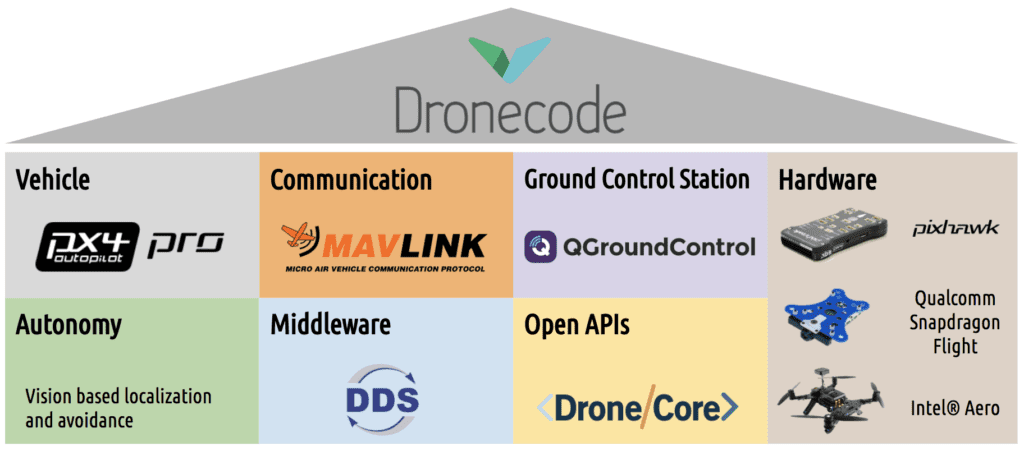
\includegraphics[width=0.8\linewidth]{./Figure/Dronecode_Software_Stack.png}
  \caption{Dronecode软硬件平台展示}\label{Fig:imgx}
\end{figure}

APM与PX4在一些关键算法上是相互借鉴的,因此算法先进程度差不多。PX4由于起步晚,历史包袱少,最初就搭建了一个很先进的架构,因此获得了代码简洁易懂易懂的优势。该开源系统在国内外影响力较大,除多旋翼外同样支持固定翼、垂直起降等机型。支持MAVLink微型空中飞行器链路通讯协议。

3.STM32/TI-嵌入式芯片飞控平台。该系列以匿名、无名飞控为主,最初是由大学生创业团队设计并开发的,具有光流定位、GPS定点等功能。只支持多旋翼系列机型,并且由于其配套地面站程序较为简易,主要适用于教学实验等领域,不适用于商业等对稳定性要求较高的环境中。对于某些特殊的机型,部分兼容MAVLink微型空中飞行器链路通讯协议。

\section{视觉检测}

根据项目需求,无人机检测地面上面的H标记采用基于OpenCV的框架,算法使用自适应阈值+形态学处理+霍夫圆检测,并返回检测的中心点,用于滤波以及后续的位置优化。

\subsection{形态学处理}

形态学处理包括开闭运算、礼帽/顶帽/黑帽、检测边和角点等。这里我们为了获取图像中的主要对象,对一副二值图连续使用闭运算和开运算。

1.腐蚀和膨胀

腐蚀的基本思想就像土壤侵蚀一样,它腐蚀了前景对象的边界(始终尝试将前景保持在白色)。它的作用为:内核在图像中滑动(如在 2D 卷积中)。仅当内核下的所有像素均为 1 时,原始图像中的像素(1 或 0)才会被视为 1,否则将被腐蚀(变为零)。

膨胀与腐蚀正好相反。此处,如果内核下的至少一个像素是“1”,则像素元素为“1”。所以它增加了图像中的白色区域或前景对象的大小增加。通常,在消除噪音的情况下,侵蚀后会扩张。因为,侵蚀可以消除白噪声,但它也会缩小我们的物体。所以我们扩张它。由于噪点消失了,它们不会再回来了,但是我们的物体面积会增加。它在连接对象的损坏部分时也很有用。

上述过程如下图所示:

\begin{figure}[ht]
  \centering
  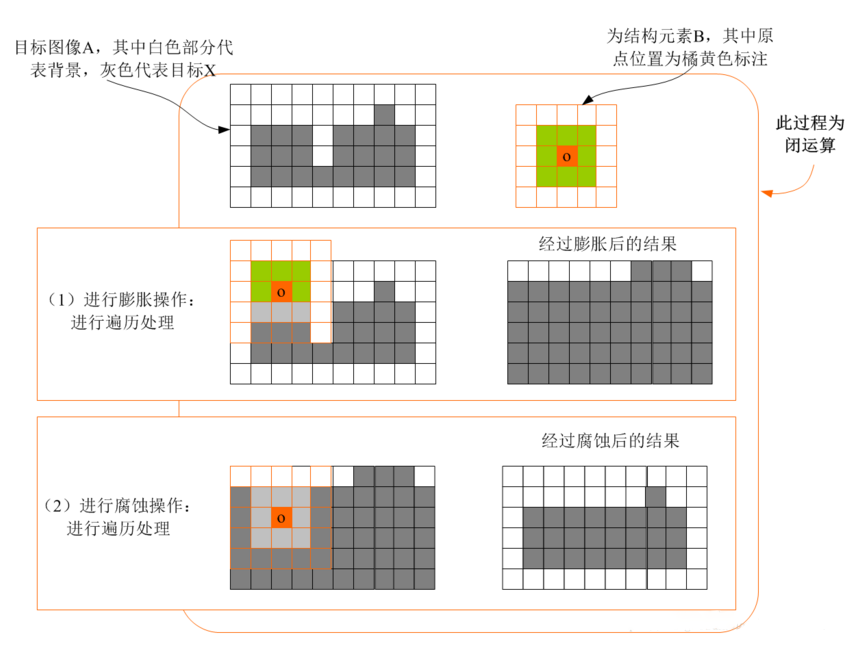
\includegraphics[width=0.8\linewidth]{./Figure/Corrosion_and_Expansion.png}
  \caption{腐蚀和膨胀变换示意}\label{Fig:img0}
\end{figure}

2.开闭运算

开运算和闭运算就是将腐蚀和膨胀按照一定的次序进行处理。但这两者并不是可逆的,即先开后闭并不能得到原先的图像。

具体流程为:

开运算:先腐蚀后膨胀,用于移除由图像噪音形成的斑点;闭运算:先膨胀后腐蚀,用来连接被误分为许多小块的对象。

OpenCV实现形态学运算的函数为:morphologyEx

该函数实现的功能是一些基于图像形状的简单操作。它通常在二进制映像上执行。它需要两个输入,一个是我们的原始图像,第二个称为结构元素或内核,它决定了操作的性质。两个基本的形态学运算符是侵蚀和扩张。然后它的变体形式,如打开,关闭,渐变等也开始发挥作用。

\subsection{霍夫圆检测}

1.霍夫变换

霍夫变换于1962年由Paul Hough首次提出,后于1972年由Richard Duda和Peter Hart推⼴使⽤,经典霍夫变换⽤来检测图像中的直线,后来霍夫变换扩展到任意形状物体的识别,多为圆和椭圆。

霍夫变换(Hough Transform, HT)是模式识别领域中对二值图像进行直线检测的有效方法\cite{Art2}。

\begin{figure}[ht]
  \centering
  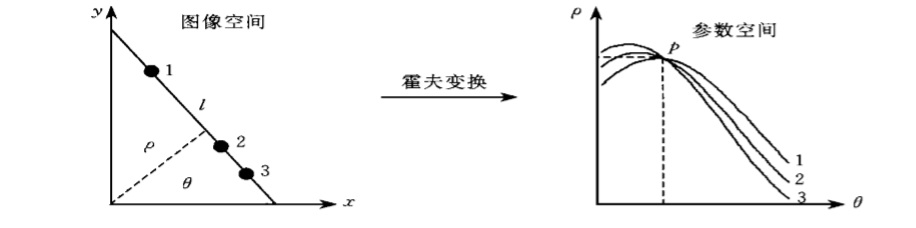
\includegraphics[width=0.8\linewidth]{./Figure/Hough_Transform.png}
  \caption{霍夫变换示意}\label{Fig:img1}
\end{figure}

在标准参数化方式下,图像空间中的直线 l 的表达为:

$d=x \cos \theta+y \sin \theta, \quad d \geqslant 0,0 \leqslant \theta<\pi$

右边的图意思是在一个点上,不同的θ对应不同的ρ,θ是穿过该点的直线的斜率,ρ是穿过该点的直线与原点的距离。这样穿过每个点作无数条直线,参数ρ和θ就能绘出一个正弦图像。 ⽽如果1,2,3在一条直线上就可以找到⼀个θ使得过1,2,3点的直线的ρ很接近。也就是有图上相交的过程。而通常使用的方法是累加法,求得累加次数最多的(θ,ρ)从⽽确定这条直线。

2.霍夫变换用于圆检测

与使用$(r, \theta)$来表示一条直线相似,使用(a,b,r)来确定一个圆心为(a,b)半径为r的圆。

某个圆过点$(x_{1}, y_{1})$,则有:$(x1-a1)^2 + (y1-b1)^2 = r1^2$

那么过点$(x_{1}, y_{1})$的所有圆可以表示为$(a_{1}(i), b_{1}(i), r_{1}(i))$,其中$r_{1} \in (0,\infty)$,每⼀个 i 值都对应⼀个不同的圆,$(a_{1}(i), b_{1}(i), r_{1}(i))$表示了无穷多个过点$(x_{1}, y_{1})$的圆。

过点$(x_{1}, y_{1})$的所有圆可以表示为$(a_{1}(i), b_{1}(i),r_{1}(i))$,过点$(x_{2}, y_{2})$的所有圆可以表示为$(a_{2}(i),b_{2}(i),r_{2}(i))$,过点$(x_{3}, y_{3})$的所有圆可以表示为$(a_{3}(i),b_{3}(i),r3(i))$,如果这三个点在同一个圆上,那么存在一个值$(a_{0},b_{0},r_{0})$,使得$a_{0} = a_{1}(k) = a_{2}(k) = a_{3}(k)$且$b_{0} = b_{1}(k) = b_{2}(k) = b_{3}(k)$且$r_{0} = r_{1}(k) = r_{2}(k) = r_{3}(k)$,即这三个点同时在圆$(a_{0}, b_{0}, r_{0})$上。

从下图可以形象的看出:

\begin{figure}[ht]
  \centering
  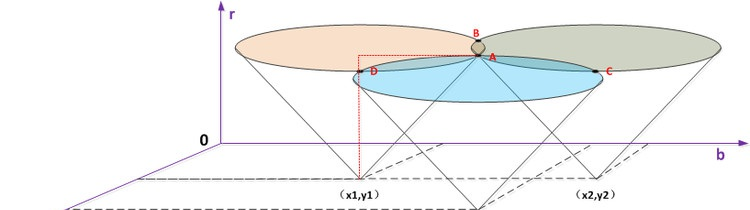
\includegraphics[width=0.8\linewidth]{./Figure/Hough_Circle.png}
  \caption{霍夫圆示意}\label{Fig:img2}
\end{figure}

⾸先,分析过点$(x_{1}, y_{1})$的所有圆$(a_{1}(i), b_{1}(i),r_{1}(i))$,当确定$(r_{1}(i)$时,$(a_{1}(i), b_{1}(i))$的轨迹是⼀个以$(x_{1}, y_{1}, r_{1}(i))$为中心半径为$r_{1}(i)$的圆。那么,所有圆$(a_{1}(i), b_{1}(i),r_{1}(i))$的组成了一个以$(x_{1}, y_{1}, 0)$为顶点,锥角为90度的圆锥面。三个圆锥面的交点A即是同时过这三个点的圆。累加次数最多的A点就是一个圆⼼。

\section{滤波优化}

对于上一步每一次检测到的降落板中心点,由于检测中存在一定的服从高斯分布的噪声,准确检测的降落点和这些噪声点同时作为参考点传入至无人机MPC位置控制中,会一定程度上导致无人机的最终位置控制存在较大的振荡与偏差,进而影响最终的降落精准度。

因此,我们需要一种有效的方法尽可能去除检测的降落点中心的高斯噪声,因此这里采用卡尔曼滤波器去除检测中心点的噪声并实现较为精确的降落点预测。

\subsection{卡尔曼滤波器}

卡尔曼滤波(Kalman filtering, KF)是一种利用线性系统状态方程,通过系统输入输出观测数据,对系统状态进行最优估计的算法\cite{ArtE3}。卡尔曼滤波的一个典型实例是从一组有限的,对物体位置的,包含噪声的观察序列中预测出物体的坐标位置及速度。在很多工程应用(雷达、计算机视觉)中都可以找到它的身影。同时,卡尔曼滤波也是控制理论以及控制系统工程中的一个重要话题。

卡尔曼滤波最早可以追溯到Wiener滤波,不同的是卡尔曼采用状态空间来描述它的滤波器,卡尔曼滤波器同时具有模糊/平滑与预测功能,特别是后者在视频分析与对象跟踪应用场景中被发扬光大,在离散空间(图像或者视频帧)使用卡尔曼滤波器相对简单。假设我们根据一个处理想知道一个变量值如下:

$x_{k+1}=\Phi x_{k}+w_{k}$

其中$x_{k}$是在$\mathrm{k}$时刻的状态,$\Phi$是从$\mathrm{k}$到$\mathrm{k}+1$时刻的变换矩阵,$w_{k}$是 $\mathrm{k}$时刻相关白噪声的协方差矩阵。

对观测值建模如下:

$z_{k}=H x_{k}+v_{k}$

其中$z_{k}$是在k时刻对x的实际测量值,$\mathrm{H}$是状态矩阵与测量矩阵无噪声链接,$\mathrm{v}_{\mathrm{k}}$ 是测量错误

这样就得到两个协方差矩阵

$$
\begin{aligned}
&Q=E\left[w_{k} w_{k}^{T}\right] \\
&R=E\left[v_{k} v_{k}^{T}\right] \\
&P_{k}=E\left[e_{k} e_{k}^{T}\right]=E\left[\left(x_{k}-\hat{x}_{k}\right)\left(x_{k}-\hat{x}_{k}\right)^{T}\right]
\end{aligned}
$$

假设$\hat{x}_{k}$前一个评估为$\hat{x}_{k}^{\prime}$, 可以得到

$$
\hat{x}_{k}=\hat{x}_{k}^{\prime}+K_{k}\left(z_{k}-H \hat{x}_{k}^{\prime}\right)
$$

其中$K_{k}$被称为卡尔曼增益, 有了它就可以更新测量模型,从而更新状态空间的下个预测。

以上流程可以用如下图示表示:

\begin{figure}[ht]
  \centering
  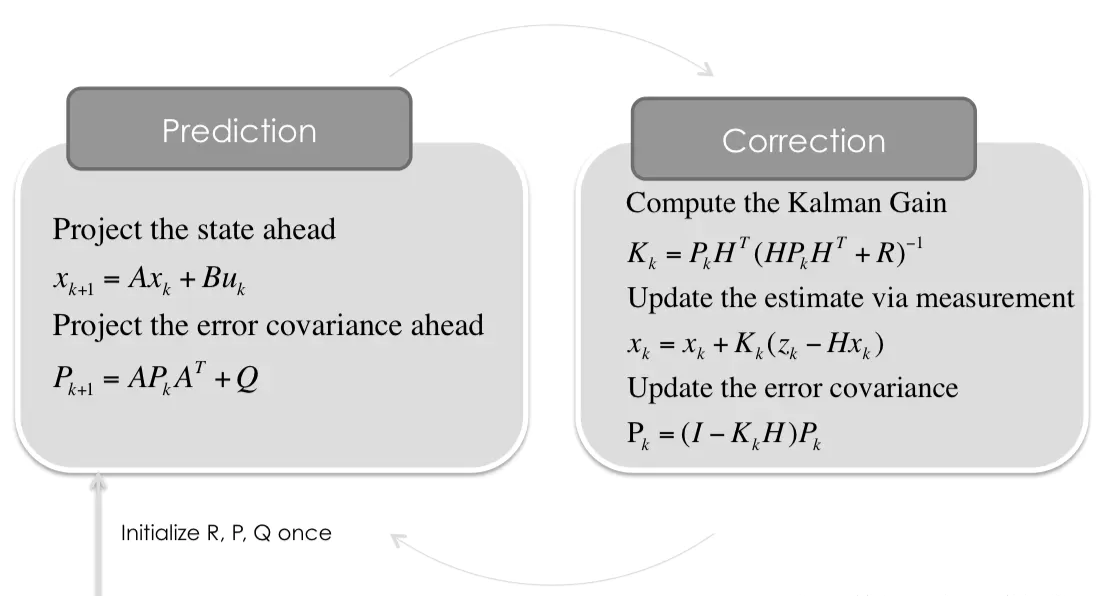
\includegraphics[width=0.8\linewidth]{./Figure/Kalman_Prediction_and_Correction.png}
  \caption{卡尔曼滤波器预测与修正}\label{Fig:img3}
\end{figure}

\section{控制算法}

根据项目需求,无人机需要在自主航点飞行完毕后自主降落至指定区域,指定降落区域地面上贴有标记为H的橙红色降落板。自主降落下降阶段我们改进了传统的基于PID的控制方案,通过采用基于MPC的控制方案对控制参数进行自适应优化,从而使得降落控制阶段更为平稳。

\subsection{PID控制}

PID控制应该算是应用非常广泛的控制算法了。小到控制一个元件的温度,大到控制无人机的飞行姿态和飞行速度等等,都可以使用PID控制。PID(proportion integration differentiation)其实就是指比例,积分,微分控制,它具有原理简单,易于实现,适用面广,控制参数相互独立,参数的选定比较简单等优点;而且在理论上可以证明,对于过程控制的典型对象──“一阶滞后+纯滞后”与“二阶滞后+纯滞后”的控制对象,PID控制器是一种最优控制\cite{ArtE2}。

\begin{figure}[ht]
  \centering
  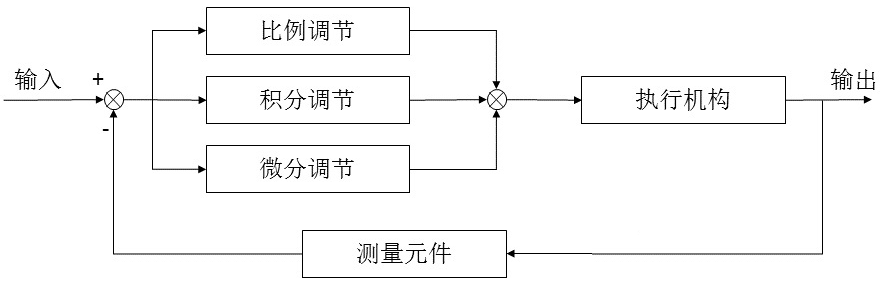
\includegraphics[width=0.8\linewidth]{./Figure/PID_Graph.png}
  \caption{PID控制系统结构图}\label{Fig:img4}
\end{figure}

根据上图所示,PID控制即为:当得到系统的输出后,将输出经过比例,积分,微分3种运算方式,叠加到输入中,从而控制系统的行为。

在工业过程中,连续控制系统的理想PID控制规律为:

$u(t)=K_{p}\left(e(t)+\frac{1}{T_{t}} \int_{0}^{t} e(t) d t+T_{D} \frac{d e(t)}{d t}\right)$

式中,Kp为比例增益,比例度成倒数关系;Tt为积分时间常数;TD为微分时间常数;u(t)为PID控制器的输出信号;e(t)为给定值r(t)与测量值之差。

针对于传统的PID控制器,其本身一般不依赖于未来的误差,这是不对的。如果依赖未来的误差,也没有考虑车辆的模型,必然不准确的控制。而对于MPC控制器来说,延迟的一个重要因素就是执行器的动态特性。例如,从转向角指令下发到实际到达该转向角度的时间。这个可以通过简单的动态系统进行建模,并且整合到车辆模型中去。一种方法就是将使用车辆模型,根据延迟时间推算延迟时间后的车辆状态,这个车辆状态就是MPC计算的新初始状态。

\subsection{MPC控制}

1.MPC控制介绍

传统PID算法的缺点是,对于系统的状态变化,控制器的输出不能很好的控制系统的状态变化,因此,在这种情况下,PID算法的效率不高。而MPC算法则是一种更好的控制方法,它能够更好的控制系统的状态变化,并且能够更好的控制系统的输出。

模型预测控制(Model predictive control、MPC)是过程控制中,在满足特定限制条件时,控制过程的进阶控制方式,自1980年代起已用在化学工厂及炼油厂的工业过程中。模型预测控制是以过程的动态模型为基础,多半是透过系统识别得到的线性经验模型。模型预测控制的特点是每一次针对目前的时间区块内作最佳化,然后下一个时间再针对时间区块内作最佳化,这和LQR控制器不同。模型预测控制可以预测未来事件并且进行对应的处理,而传统的PID控制器没有这样的预测功能。预测控制打破了传统控制中对模型结构的严格要求,更着重于在系统已获取的信息的基础上根据功能要求按照最方便的途径建立模型。尽管模型预测控制形式多种多样,但都依赖下述三项基本原理:

1.1 预测模型

预控制是一种基于模型的控制算法,这一校型称为预测模型\cite{Art3}。对于预测控制来讲,只注重模型的功能,而不注重模型的形式,预测模型的功能就是能根据对象的历史信息和未来输入预其未来输出。从方法的角度讲,只要是具有预测功能的信息集合,不论其有什么样的表现形式,均可作为预测模型。因此,状态方程,传递函数这类传统的模型都可以作为预测模型。

1.2 滚动优化

预测控制的最主要特征是在线优化。预测控制这种优化控制算法是通过某一性能指标的最优来确定未来的控制作用的。这一性能指标涉及到系统未来的行为,例如,通常可取对象输出在未来的采样点上跟踪某一期望轨迹的方差最小.但也可取更广泛的形式,要求控制能量为最小而同时保持输出在某一给定范围内等。性能指标中涉及到的系统未来的行为,是根据预测模型由未来的控制策略决定的\cite{ArtE8}。

1.3 反馈校正

预控制算法在进行滚动优化时,优化的基点应与系统实际一致。但作为基础的预测模型,只是对象动态特性的粗略描述,由于实际系统中存在的非线性、时变、模型失配、干扰等因素,基于不变模型的预测不可能和实际情况完全相符,这就需用要用附加的预测手段补充模型预的不足,或者对基础模型进行在线峰正\cite{Art4}。滚动优化只有建立在反馈校正的基础上,才能体见出其优越性。因此,预测控制算法在通过优化确定了一系列末来的控制作用后,为了防止模型失配或环境干扰引起控制对理想状态的偏离,并不是把这些控制作用逐一全部实施,而只是实现本时刻的控制作用\cite{Art5}。到下一采样时刻,则首先检测对象的实际输出,并利用这一实时信息对基于模型的预测进行修正,然后再进行新的优化\cite{ArtE6}。

以下方框图提供了MPC原理的可视化表示:

\begin{figure}[ht]
  \centering
  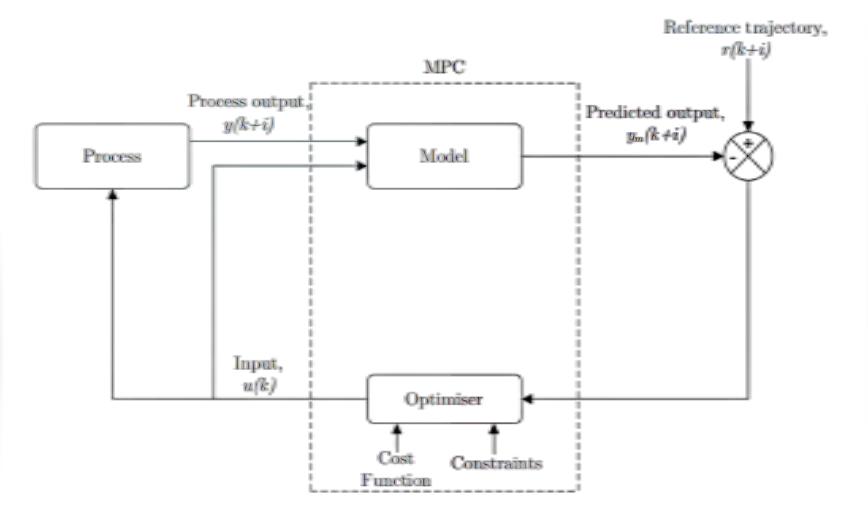
\includegraphics[width=0.8\linewidth]{./Figure/MPC-Control.png}
  \caption{MPC控制系统结构图}\label{Fig:img5}
\end{figure}

以下图说明了MPC中的预测范围:

\begin{figure}[ht]
  \centering
  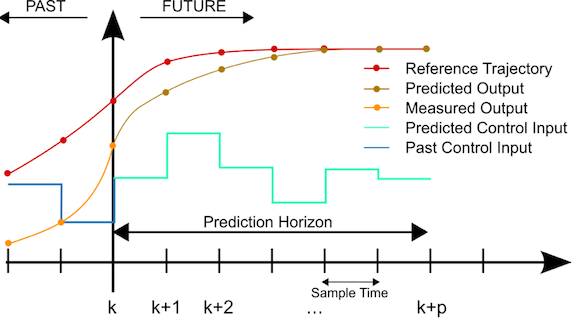
\includegraphics[width=0.8\linewidth]{./Figure/MPC-Prediction.png}
  \caption{MPC预测范围}\label{Fig:img6}
\end{figure}

2.MPC控制系统控制器建模

对于以下控制模型:

$$
x(k+1)=A x(k)+B u(k)
$$

写成矩阵格式:

$$
\left[\begin{array}{l}x_{1}(k+1) \\x_{2}(k+1)\end{array}\right]=\left[\begin{array}{cc}1 & 0.1 \\0 & 2\end{array}\right]\left[\begin{array}{l}x_{1}(k) \\x_{2}(k)\end{array}\right]+\left[\begin{array}{c}0 \\0.5\end{array}\right] u(k)
$$

此处的$x_{1}$和$x_{2}$可以理解为误差项

$X(k)=\left[\begin{array}{c}x(k \mid k) \\x(k+1 \mid k) \\\vdots\\ x(k+j \mid k)\\\vdots \\x(k+N \mid k)\end{array}\right]$$U(k)=\left[\begin{array}{c}u(k \mid k) \\u(k+1 \mid k) \\\vdots\\ u(k+i \mid k)\\\vdots \\u(k+N-1 \mid k)\end{array}\right]$

对于MPC矩阵:

$$
x_{k}=M x_{k}+C u_{k}
$$

$$
M=\left[\begin{array}{c}I_{n \times n} \\A_{n \times n} \\A_{n}^{2} \\\vdots \\A^{N}\end{array}\right]
$$

$$
C=\left[\begin{array}{cccc}
0 & 0 & \ldots & 0 \\
& \vdots & \ldots & \vdots \\
\vdots & 0 & & 0 \\
0 & 0 & \ldots & 0 \\
B_{n \times p} & 0 & \ldots & 0 \\
A B_{n \times p} & B & \vdots & 0 \\
\vdots & \vdots & & B
\end{array}\right]
$$

$X(k)=\left[\begin{array}{c}x(k \mid k) \\x(k+1 \mid k) \\x(k+2 \mid k) \\x(k+3 \mid k)\end{array}\right]=\left[\begin{array}{c}x_{1}(k \mid k) \\x_{2}(k \mid k) \\x_{1}(k+1 \mid k) \\x_{2}(k+1 \mid k) \\x_{1}(k+2 \mid k) \\x_{2}(k+2 \mid k) \\x_{1}(k+3 \mid k) \\x_{2}(k+3 \mid k)\end{array}\right]$

$U(k)=\left[\begin{array}{c}u(k \mid k) \\u(k+1 \mid k) \\u(k+2 \mid k)\end{array}\right]=\left[\begin{array}{c}\frac{u(k \mid k)}{u(k+1 \mid k)} \\u(k+2 \mid k)\end{array}\right]$

计算出M矩阵和C矩阵

之后构建二次规划模式(cost function)\cite{ArtE7}

$$
J=\sum_{k=0}^{N-1} x(k+i \mid k)^{T} Q x(k+i \mid k)+u(k+i \mid k)^{T} R u(k+i \mid k)+x(k+N \mid k)^{T} F x(k+i \mid k)
$$

Q、R、F表示对应输入输出的权重系数矩阵

Q矩阵影响x变量的相关性,R矩阵跟输入相关,F矩阵跟终值相关

$x(k+N \mid k)^{T} F x(k+i \mid k)$与系统对应的终值状态相关

简化上面的cost function矩阵

$$
J=\boldsymbol{x}(k)^{T} \boldsymbol{G} \boldsymbol{x}(k)+\boldsymbol{U}(k)^{T} \boldsymbol{H} \boldsymbol{U}(k)+2 \boldsymbol{x}(k)^{T} \boldsymbol{E} \boldsymbol{U}(k)
$$

该矩阵只包含了输入项和已知的初始输入项x(k)

$$
\begin{aligned}&G=M^{T} \bar{Q} M \\&E=C^{T} \bar{Q} M \\&H=C^{T} \bar{Q} C+\bar{R}\end{aligned}
$$

$\bar{Q}$和$\bar{R}$表示上面式子中的Q和R矩阵的增广形式

G、H、E矩阵跟上面的M和C矩阵相关

$$
\overline{\boldsymbol{Q}}=\left[\begin{array}{ccc}\boldsymbol{Q} & \cdots & \\\vdots & \boldsymbol{Q} & \vdots \\& \cdots & \boldsymbol{F}\end{array}\right] \quad \overline{\boldsymbol{R}}=\left[\begin{array}{ccc}\boldsymbol{R} & \cdots & \\\vdots & \ddots & \vdots \\& \cdots & R\end{array}\right]
$$

\subsection{MAVLink协议}

Mavlink协议最早由苏黎世联邦理工学院 计算机视觉与几何实验组 的 Lorenz Meier于2009年发布,并遵循LGPL开源协议。Mavlink协议是在串口通讯基础上的一种更高层的开源通讯协议,主要应用在微型飞行器(micro aerial vehicle)的通讯上。Mavlink是为小型飞行器和地面站(或者其他飞行器)通讯时常常用到的那些数据制定一种发送和接收的规则并加入了校验(checksum)功能\cite{ArtE4}。

Mavlink传输时的基本单位是消息帧,以下为消息帧的结构。

\begin{figure}[ht]
  \centering
  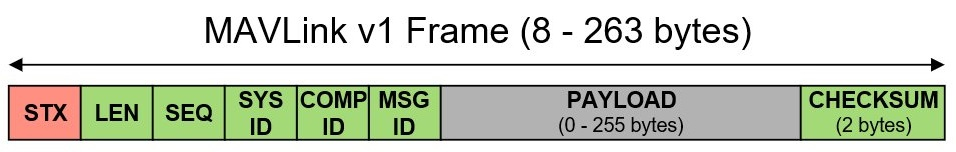
\includegraphics[width=0.8\linewidth]{./Figure/Mavlink_Frame.jpg}
  \caption{MAVLink Frame}\label{Fig:img7}
\end{figure}

如上图所示,每个消息帧都是上述的结构,除了灰色外,其他的格子都代表了一个字节的数据。

红色的是起始标志位(stx),在v1.0版本中以“FE”作为起始标志。这个标志位在mavlink消息帧接收端进行消息解码时有用处。

第二个格子代表的是灰色部分(payload,称作有效载荷,要用的数据在有效载荷里面)的字节长度(len),范围从0到255之间。在mavlink消息帧接收端可以用它和实际收到的有效载荷的长度比较,以验证有效载荷的长度是否正确。

第三个格子代表的是本次消息帧的序号(seq),每次发完一个消息,这个字节的内容会加1,加到255后会从0重新开始。这个序号用于mavlink消息帧接收端计算消息丢失比例用的,相当于是信号强度。

第四个格子代表了发送本条消息帧的设备的系统编号(sys),使用PIXHAWK刷PX4固件时默认的系统编号为1,用于mavlink消息帧接收端识别是哪个设备发来的消息。

第五个格子代表了发送本条消息帧的设备的单元编号(comp),使用PIXHAWK刷PX4固件时默认的单元编号为50,用于mavlink消息帧接收端识别是设备的哪个单元发来的消息(暂时没什么用) 。

第六个格子代表了有效载荷中消息包的编号(msg),注意它和序号是不同的,这个字节很重要,mavlink消息帧接收端要根据这个编号来确定有效载荷里到底放了什么消息包并根据编号选择对应的方式来处理有效载荷里的信息包。

最后两个字节是16位校验位,ckb是高八位,cka是低八位。校验码由crc16算法得到,算法将整个消息(从起始位开始到有效载荷结束,还要额外加上个MAVLINK\_CRC\_EXTRA字节)进行crc16计算,得出一个16位的校验码。之前提到的每种有效载荷里信息包(由消息包编号来表明是哪种消息包)会对应一个MAVLINK\_CRC\_EXTRA,这个 MAVLINK\_CRC\_EXTRA 是由生成mavlink代码的xml文件生成的,加入这个额外的东西是为了当飞行器和地面站使用不同版本的mavlink协议时,双方计算得到的校验码会不同,这样不同版本间的mavlink协议就不会在一起正常工作,避免了由于不同版本间通讯时带来的重大潜在问题。

MAVLink帧的介绍如下图所示:

\begin{figure}[ht]
  \centering
  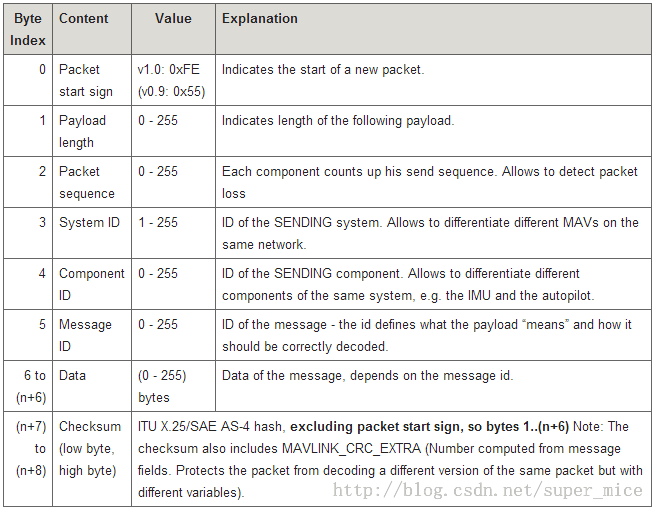
\includegraphics[width=0.8\linewidth]{./Figure/Mavlink_Frame_Intro.png}
  \caption{MAVLink Frame介绍}\label{Fig:img8}
\end{figure}

在MAVLink消息帧中最重要的两个内容:一个是msgid,一个是payload,前者是payload中内容的编号,后者则存放了消息。消息有许多种类型,在官网的网页中中以蓝色的“\#”加数字的方式来表示消息的编号如 “\#0”。

由于DJI MSDK协议本身不存在与MAVLink的兼容,因此我们针对于开源项目的MAVLink协议部分进行转换,根据实际项目控制的需要进行适配兼容MAVLink部分协议,并未完全兼容MAVLink支持的所有协议。

\chapter{项目内容}

\section{项目概要}

本项目使用大疆御2行业进阶版无人机作为主体,基于DJI MSDK进行二次开发,对DJI MSDK自有的协议转换为兼容QGC地面站的MAVLink协议,并通过无人机端侧带屏遥控器通过以太网数据链路远程组网传输信息至远端的QGC地面站软件,以及可见光和热成像视频流信息。无人机根据地面站给出的航点信息完成航点飞行,任务结束后,云台自动向下旋转90度,并利用OpenCV计算机视觉库完成自适应阈值+形态学处理+霍夫圆检测,并使用MPC控制算法完成自主视觉引导降落至特定降落目标点。

\section{APP整体框架}

本项目基于开源代码rosettadrone进行二次开发,在Android源代码的基础上单独添加了OpenCV检测框架以及MPC位置控制器设计部分。Rosetta Drone是DJI SDK的Mavlink包装器,允许用户使用Mavlink语言的地面控制站控制DJI无人机。从理论上讲,它应该与任何Mavlink GCS一起使用,但到目前为止,我们所有测试都是使用QGroundControl完成的。

APP集成的功能:

1.在QGC中报告遥测数据,如位置、姿态、相对高度、航向和电池剩余电量

2.从QGC返回启动的命令

3.在QGC中查看无人机视频源或将RTP转发到您选择的IP地址

4.创建和飞行航点任务

5.通过操纵杆和QGS飞行

6.从DroneKit中的 Python 起飞

7.使用Mavproxy同时连接QGC和DroneKit

8.使用Gstreamer/OpenCV/FFMPEG和DroneKit创建复杂的AI功能

飞行任务流程:

1.将无人机配套的带屏遥控器打开,然后打开DJI无人机的电源。

2.启动Rosetta Drone APP。如果应用程序成功与您的无人机通信,右上角的DJI灯将变为绿色。

3.如果需要在外部设备上使用 QGroundControl,单击齿轮图标以访问“设置”,选中“在外部设备上使用 GCS”,然后指定 IP 地址。

4.启动QGroundControl。应立即建立遥测连接,Rosetta Drone 中的 GCS 指示灯将变为绿色。请注意,如果在与Rosetta无人机相同的设备上使用QGroundControl,则如果QGC在背景中,GCS灯可能不会变为绿色。

5.UDP视频回传步骤:

a.点击QGC左上角的“Q”图标

b.在“视频”下,将“视频源”更改为“UDP 视频流”。

c.将UDP端口更改为 5600。

6.为确保飞行安全,建议使用遥控器手动起飞。要从 GCS 解锁并起飞,需要单击“安全启用”按钮。它将变为绿色,并显示“准备飞行”。然后使用QGroundControl起飞或启动任务功能。

7.飞行后,确保在接近无人机之前启用安全开关。

\section{OpenCV视觉检测}

使用DJI的codecManager函数获取H.264的RGBA原始视频,并将获取到的每一帧新建一个Mat类型的矩阵,用于后续处理。之后利用cvtColor函数将该帧图像的RGB色彩通道转化为灰度图像,之后进行闭运算并利用findContours函数寻找图像的轮廓,寻找到轮廓后,利用drawContours函数将轮廓绘制出来,最后将图像转化为Mat类型的矩阵,并将其存入一个vector类型的容器中,最后进行霍夫圆检测。

OpenCV实现的是一个比标准霍夫圆变换更为灵活的检测方法——霍夫梯度法,该方法运算量相对于标准霍夫圆变换大大减少。其检测原理是依据圆心一定是在圆上的每个点的模向量上,这些圆上点模向量的交点就是圆心,霍夫梯度法的第一步就是找到这些圆心,这样三维的累加平⾯就又转化为二维累加平面。第二步是根据所有候选中心的边缘非0像素对其的支持程度来确定半径。

具体实现方法如下:

1.对于drawContours函数绘制的边缘图像,对其中的每一个非零点,考虑其局部梯度,即用Sobel()函数计算x和y方向的Sobel⼀阶导数得到梯度。

2.利用得到的梯度,由斜率指定的直线上的每一个点都在累加器中被累加,这⾥的斜率是从一个指定的最小值到指定的最大值的距离。

3.同时,标记边缘图像中每一个非0像素的位置。

4.然后从二维累加器中这些点中选择候选的中心,这些中心都大于给定阈值并且大于其所有近邻。这些候选的中心按照累加值降序排列,以便于最支持像素的中心首先出现。

5.接下来对每⼀个中心,考虑所有的非0像素,并把这些像素按照其与中心的距离排序。从到最大半径的最小距离算起,选择非0像素最支持的⼀条半径\cite{Art6}。

6.如果⼀个中心收到边缘图像⾮0像素最充分的支持,并且到前期被选择的中心有足够的距离,那么它就会被保留下来。

\section{卡尔曼滤波与优化}

OpenCV中有两个版本的卡尔曼滤波方法:KalmanFilter(C++)和CvKalman,这里我们使用前者方案。由上一步逐帧检测得到的中心点作为待估计的状态点传入卡尔曼滤波器中,并将最优估计后的结果传出作为MPC控制的输入。

卡尔曼滤波器具体实现方法如下:

1.初始化相关参数:根据需要,定义转移矩阵A与测量矩阵H,过程噪声Q与测量噪声R,最小均方误差P,系统初始状态x(0)与初始测量值z(0)

2.预测模型:利用KF.predict()函数,返回的是下一时刻的状态值KF.statePost(k+1)

3.更新上一步的测量值measurement

4.更新卡尔曼增益量KF.correct(measurement),最终的结果应该是更新后的状态估计statePost

以上流程用流程图表示为:

\begin{figure}[ht]
  \centering
  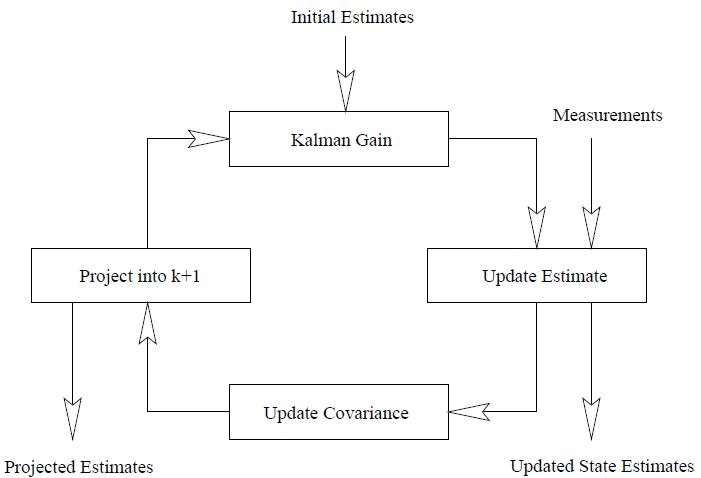
\includegraphics[width=0.8\linewidth]{./Figure/Kalman_Filter_Code_Process.jpeg}
  \caption{Kalman滤波器工作流程}\label{Fig:img9}
\end{figure}

\section{MPC位置控制}

我们提出的四轴飞行器模型预测器位置控制如下图方框中所示:

\begin{figure}[ht]
  \centering
  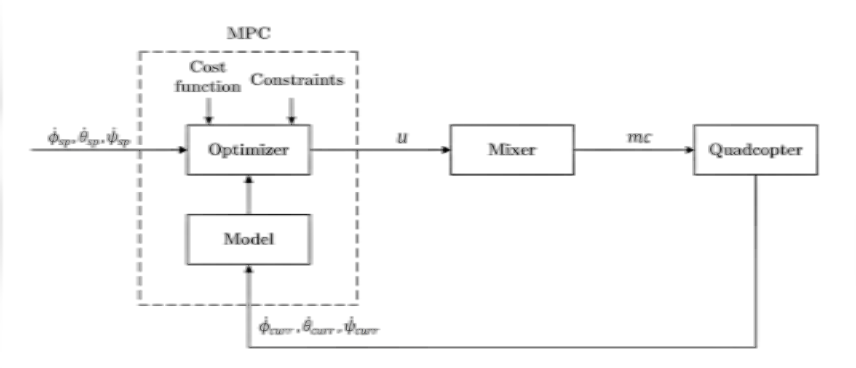
\includegraphics[width=0.8\linewidth]{./Figure/MPC-Diagram.png}
  \caption{MPC控制过程图}\label{Fig:img10}
\end{figure}

在MPC控制中,每个优化回路开始前,使用四轴飞行器状态空间模型来增强当前的角速率(这里由于MSDK API设定,认为角速率近似等于对应的虚拟摇杆控制的速率,我们使用虚拟摇杆进行控制)。这样做是为了获得更精确的四轴飞行器状态预测并用于优化器。使用这种方法可以确保在建模过程中做出的模型的不确定性和假设得到补偿\cite{ArtE1}。

速率设定点从姿态控制器发送到优化器块。优化器还接收成本函数和系统约束。希尔德雷斯的二次规划程序被用于优化器块,以最小化受预定义的四轴飞行器约束的成本函数。MPC控制器的输出是控制或输入向量u。在将这个向量发布到DJI虚拟摇杆控制之前,在-1和1之间进行缩放;这种形式的缩放是针对于DJI虚拟摇杆控制的要求。最终将缩放后的向量发送到混控器中用于最终的四旋翼位置控制。

\section{MAVLink遥控器端与QGC地面站通信过程}

APP在在连接上地面站后会主动向地面站发送心跳包(HEARTBEATS),飞行器姿态,系统状态,遥控器信号等组成的数据流。各个数据都会以一定的频率发送,心跳包发送频率为1Hz,姿态信息频率为7-8Hz,采用UDP VPN组网连接QGC时的姿态数据发送频率在7-8Hz左右。QGC地面站会在刚连接上遥控器时发送命令,请求飞控传回所有参数,飞控根据自己的情况判断是否接受地面站的请求,并根据不同的命令执行相应的操作,针对于一些特殊命令需要飞控回复地面站确认信号。之后地面站根据用户的操作会发送相应的mavlink消息给飞控,比如设置航点,解锁起飞等。整个通信过程采用半双工方式(在同一时刻只能选择发送或者选择接受数据,不能同时收发数据)\cite{ArtE5}。

以上UDP通信的内容可以通过Wireshark软件进行抓包分析,由于数据包为原始信息,难以直接辨认其数据帧的内容,因此我们使用MAVLink Lua脚本(mavgen)对数据帧的内容进行解析与类别对应。以下为解析后的数据帧内容:

\begin{figure}[ht]
  \centering
  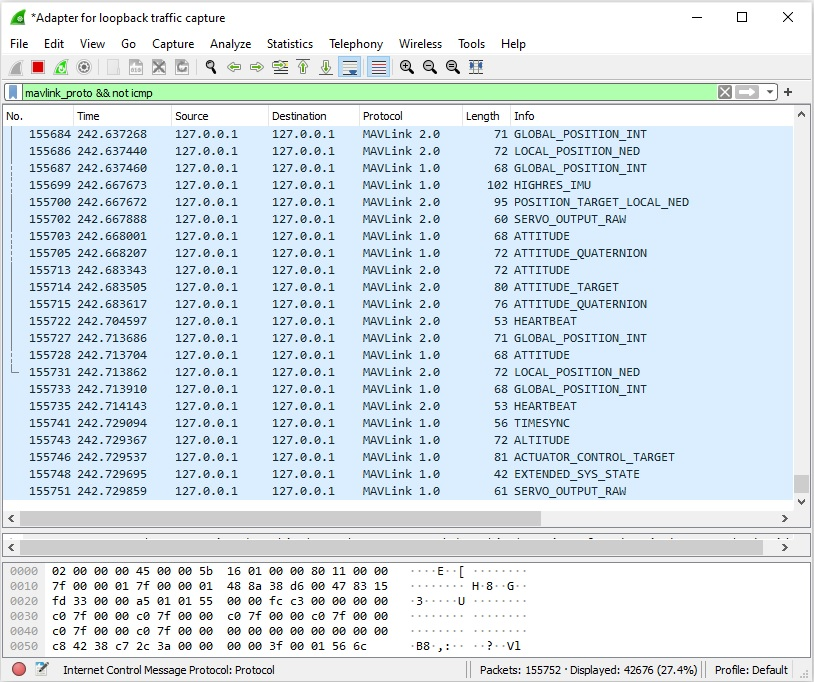
\includegraphics[width=0.8\linewidth]{./Figure/Mavlink_Wireshark_Decode.jpg}
  \caption{Wireshark MAVLink数据抓包解析}\label{Fig:img11}
\end{figure}

MAVLink支持多种飞行模式,比如manual(手动)模式、auto(自动)模式、althold(定高)模式、posctl(位置)模式、guided(外部引导控制)等。这里我们仅使用guided模式作为地面站控制模式,manual模式作为摇杆控制的手动飞行模式,如下图所示:

\begin{figure}[ht]
  \centering
  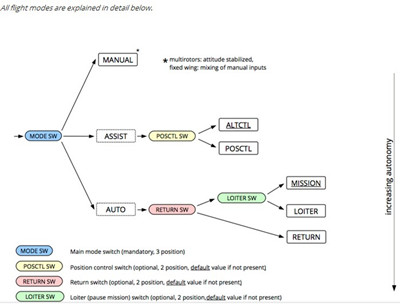
\includegraphics[width=0.8\linewidth]{./Figure/Flight_Mode.png}
  \caption{MAVLink 飞行模式图}\label{Fig:img12}
\end{figure}

这里由于我们使用QGC地面站外部控制航点飞行,因此我们选用guided模式作为地面站控制模式。

\chapter{实验结果}

我们使用蒲公英4G VPN室外工业路由器广播5.8G WiFi信号,并WiFi连接带屏遥控器端,并在地面站端侧安装蒲公英客户端,并设置路由器端与地面站软件端连接至同一虚拟网络中,使得地面站端可以与遥控器端侧通过虚拟局域网通信。在此基础上,我们使用QGroundControl开源地面站软件,并在APP中配置MAVLink UDP目的地址IP,端口14550,地面站QGC端配置MAVLink UDP端口同样为14550,如下图所示:

\begin{figure}[ht]
  \centering
  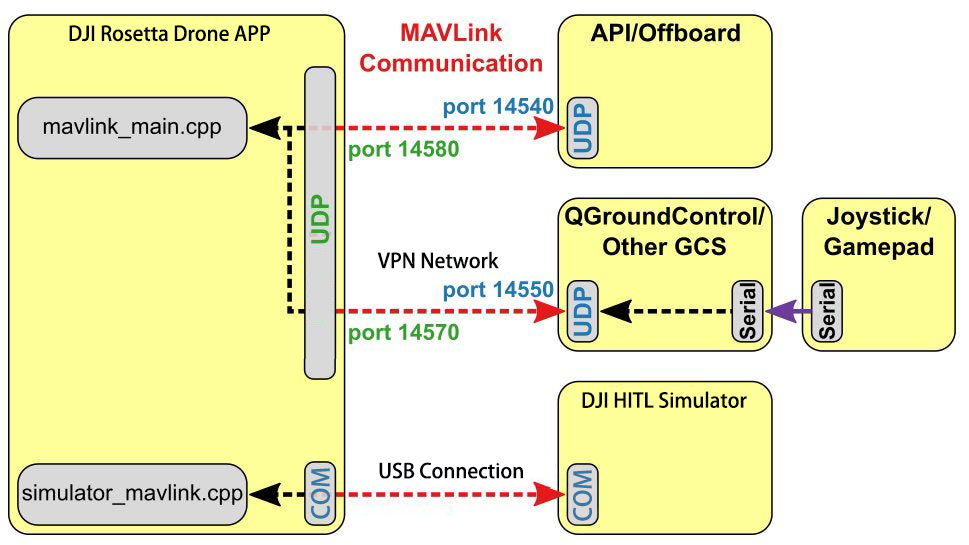
\includegraphics[width=0.8\linewidth]{./Figure/QGC_Connect_to_APP.png}
  \caption{QGC地面站网络连接至APP}\label{Fig:img13}
\end{figure}

连接配置成功后可以在地面端看到对应的电量显示以及信号强度显示。

以下为APP的飞行主界面展示:

\begin{figure}[ht]
  \centering
  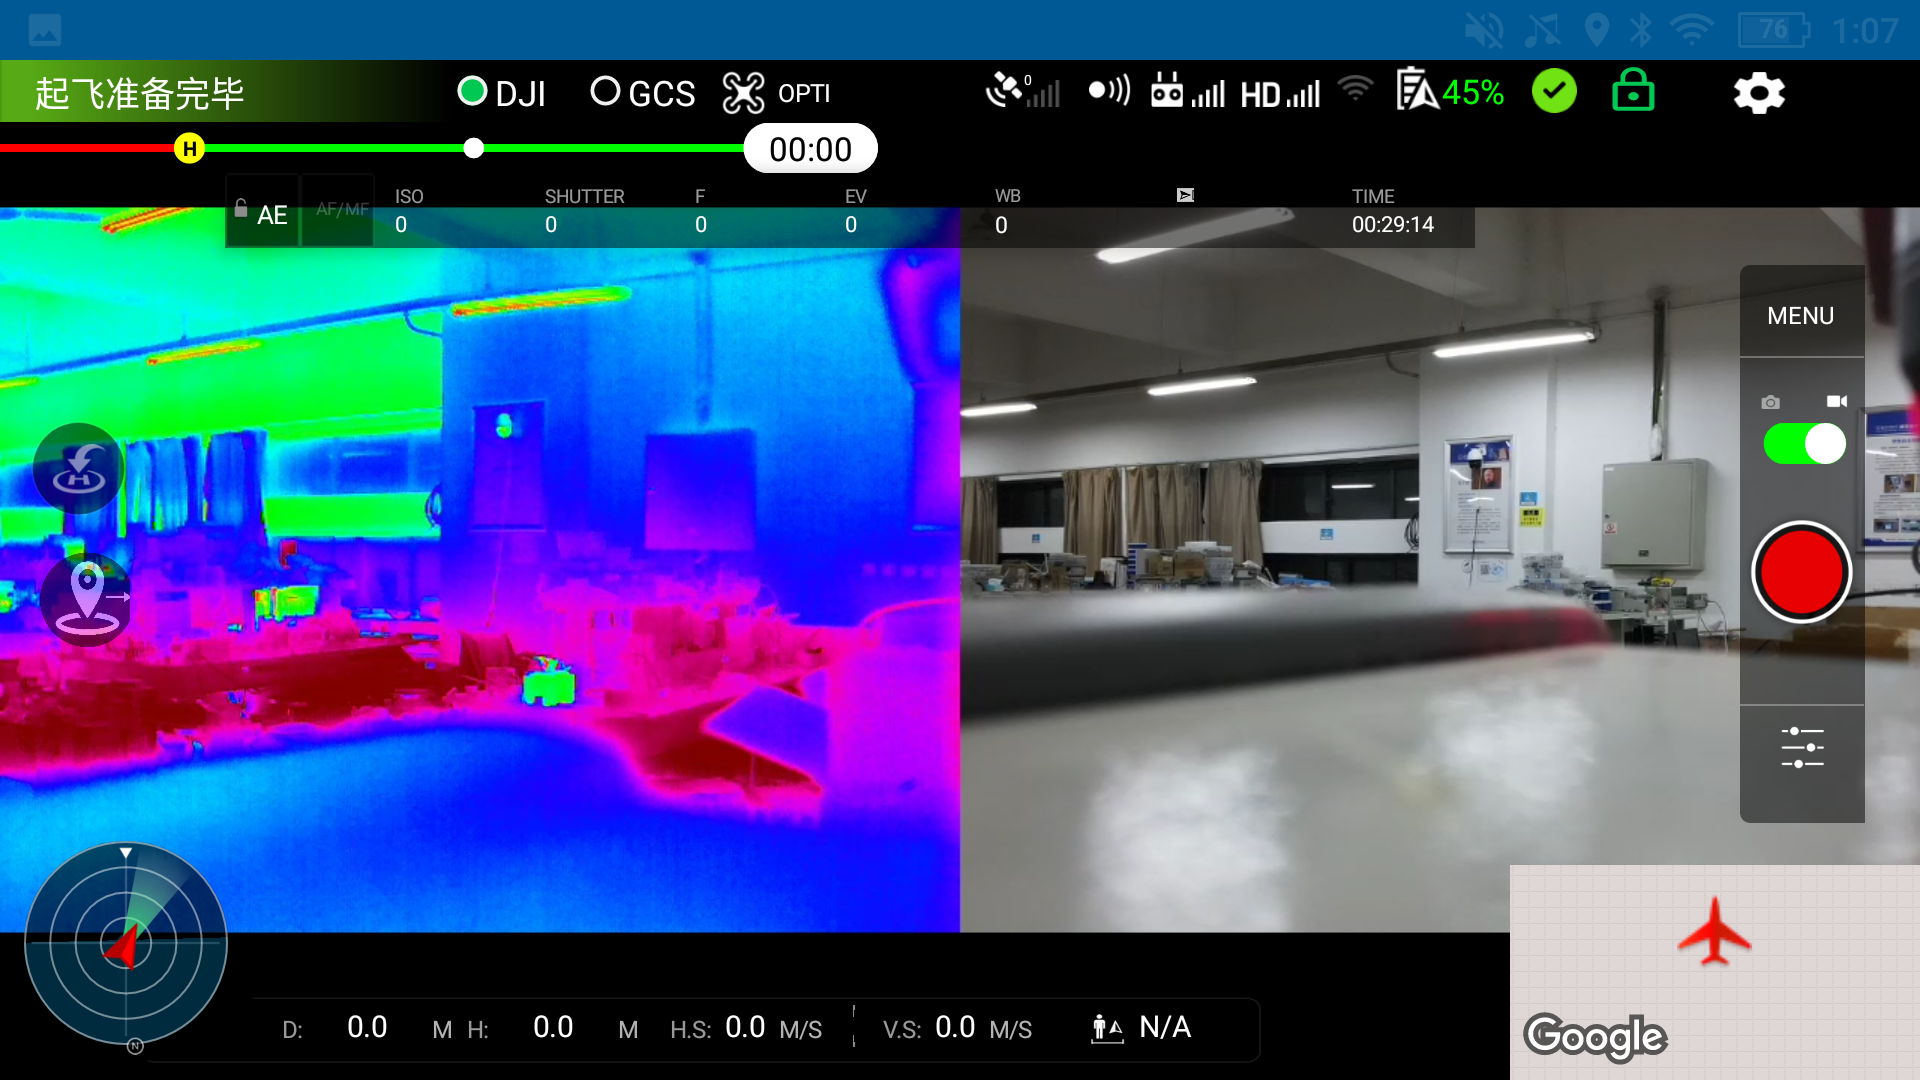
\includegraphics[width=0.8\linewidth]{./Figure/APP_Main_Page.png}
  \caption{APP主界面}\label{Fig:img14}
\end{figure}

QGC地面站MAVLink回传显示:

\begin{figure}[ht]
  \centering
  \includegraphics[width=0.8\linewidth]{./Figure/QGC_Main_Page.png}
  \caption{APP主界面}\label{Fig:img15}
\end{figure}

由于无人机室外飞行存在较大的不确定性,为避免炸机造成损失,我们使用了DJI提供的DJI Assistant 2 for Mavic软件实现了硬件在环仿真(HITL Simulation)。与此同时,我们在带屏遥控器的APP中集成了基于虚拟摇杆输入控制的DJI Simulator,并实现了APP内的软件在环仿真(SITL Simulation)。

根据实际的多次项目试飞测试,我们进行了以下的优化处理:

使用DJI飞行器传回的原始H.264视频数据进行检测处理,每帧图像耗时100ms~150ms,实时性较低,因此我们一定程度上降低了原始的H.264视频图像分辨率。

优化了无人机的控制轨迹模型,定义了更为合适的代价函数(cost function)用于将预测的输出驱动到所期望的参考值。该方法可以在样本时间k时,根据预测范围的大小生成输出预测。

\section{OpenCV视觉检测效果}

原始1080P H.264编码格式的视频逐帧处理所需时间在100ms~150ms之间,帧率约为6.7fps~10fps,难以满足实时检测的要求,而且由于该帧率下对应的控制频率在5Hz~10Hz之间,相较于期望控制频率20Hz~30Hz较低,使用PID+MPC算法进行xy位置控制存在较大的肉眼可见的比例控制振荡现象,因此我们将分辨率由1920x1080等比缩小并降低至568x320,此时的检测帧率可提升至25fps~35fps,对应的控制频率可提升至20Hz~30Hz,该控制频率下无人机的xy位置控制振荡现象明显减少,而且控制过程更为柔和。

根据二值化的阈值参数不同,以及调整霍夫圆检测中的圆心与圆心间的距离,图像中的圆的大小设置,最终将检测效果进行了一些相关优化,以下为最终的降落板识别效果:

\begin{figure}[ht]
  \centering
  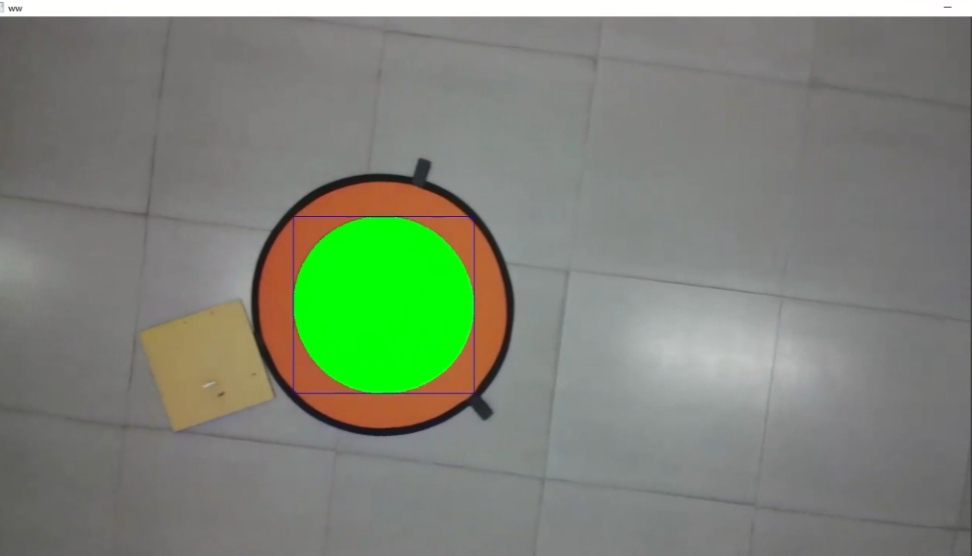
\includegraphics[width=0.8\linewidth]{./Figure/Hough_Circle_Detection.png}
  \caption{霍夫圆检测效果}\label{Fig:img16}
\end{figure}

\section{MPC模型预测控制效果}

我们使用MATLAB对模型进行理想化仿真,并在APP上集成了MPC模型控制器。正弦函数为用作控制器要跟踪的引用。它的性能是通过将模型输出(或响应)与参考一起绘制,通过改变控制和预测范围来观察。以上的权重对控制输入进行了调整,以适应这些变化。此外,适用的矩阵和向量取决于控制和预测的大小范围,被修改为兼容的矩阵和矢量计算。

MPC角速率控制器跟踪的正弦参考是下面的傅里叶级数

$$
\left[\begin{array}{c}
\dot{\phi} \\
\dot{\theta} \\
\dot{\psi}
\end{array}\right]=\left[\begin{array}{c}
\sin t+\frac{\cos (3 t)}{2} \\
\sin t+\frac{\cos (3 t)}{2} \\
\sin t+\frac{\cos (2 t)}{2}+\frac{\sin (3 t)}{3}
\end{array}\right]
$$

变量$\dot{\phi}$、$\dot{\theta}$和$\dot{\psi}$是滚动、俯仰和偏航的角速率轴分别以弧度/秒为单位测量,t是模拟时间步长,其为
边界在0和20之间;增量为0.2。

下表显示了MATLAB模拟需要初始化的参数,其中$\left[\begin{array}{lll}p & q & r\end{array}\right]^{T}=\left[\begin{array}{lll}\dot{\phi} & \dot{\theta} & \dot{\psi}\end{array}\right]^{T}$,$n_{u}=3, n_{y}=6$

\begin{tabular}{|c|c|c|c|c|}
  \hline$n_{u}$ & $n_{y}$ & $\mathbf{p}, \mathbf{q}$ & $\mathbf{r}$ & disturbance \\
  \hline 3 & 6 & $\operatorname{sint}+\frac{\cos (3 t)}{2}$ & $\operatorname{sint}+\frac{\cos (2 t)}{2}+\frac{\sin (3 t)}{3}$ & $(\operatorname{rand}(3,101) * 2-1) * 0.5$ \\
  \hline
\end{tabular}

为了验证MPC模型预测控制的效果,我们通过最小化过程通过封装Hildreth的二次规划函数和状态空间模型参数来减缓,在向混控器模块输出输入(或扭矩)命令之前至少运行两次。运行三次循环导致四轴飞行器在起飞后偏离航线,随后坠毁。然而,一个带有两次迭代的循环导致了通过每个任务路径点的相对平稳的飞行,并且任务以一个安全着陆结束。

下面绘制的飞行数据中使用的控制视野和预测视野分别为2和4。

\begin{figure}[ht]
  \centering
  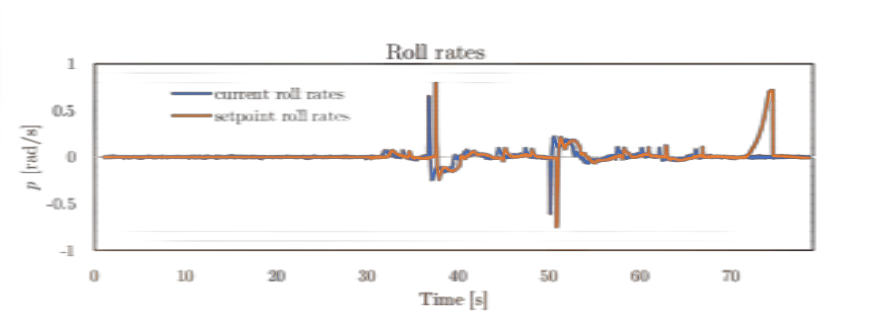
\includegraphics[width=0.8\linewidth]{./Figure/MPC-Roll-Rates.png}
  \caption{MPC滚转速率曲线}\label{Fig:img17}
\end{figure}

\begin{figure}[ht]
  \centering
  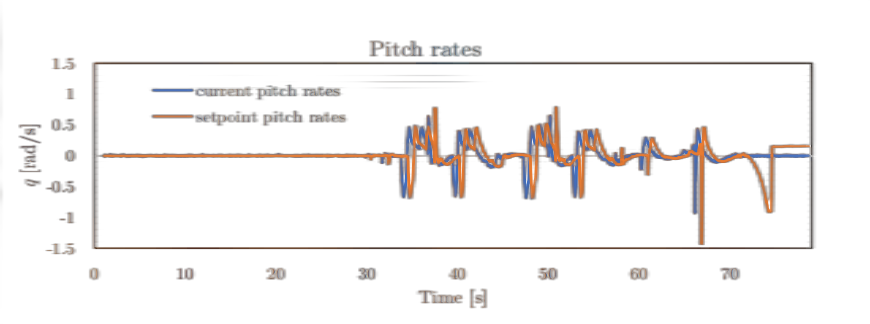
\includegraphics[width=0.8\linewidth]{./Figure/MPC-Pitch-Rates.png}
  \caption{MPC俯仰速率曲线}\label{Fig:img18}
\end{figure}

\section{降落点精准度评价}

未使用卡尔曼滤波器的降落点检测,无人机降落落点精度为:-15cm\~15cm。

通过算法的优化与改进,以及添加了卡尔曼滤波器的最优估计,可以使无人机最终降落精度达到-5cm\~5cm。

下图展示了使用卡尔曼滤波器进行降落点最优估计的检测效果:(绿色的圆点表示预测的位置,其中该圆点的圆心表示预测的中心坐标)

\begin{figure}[ht]
  \centering
  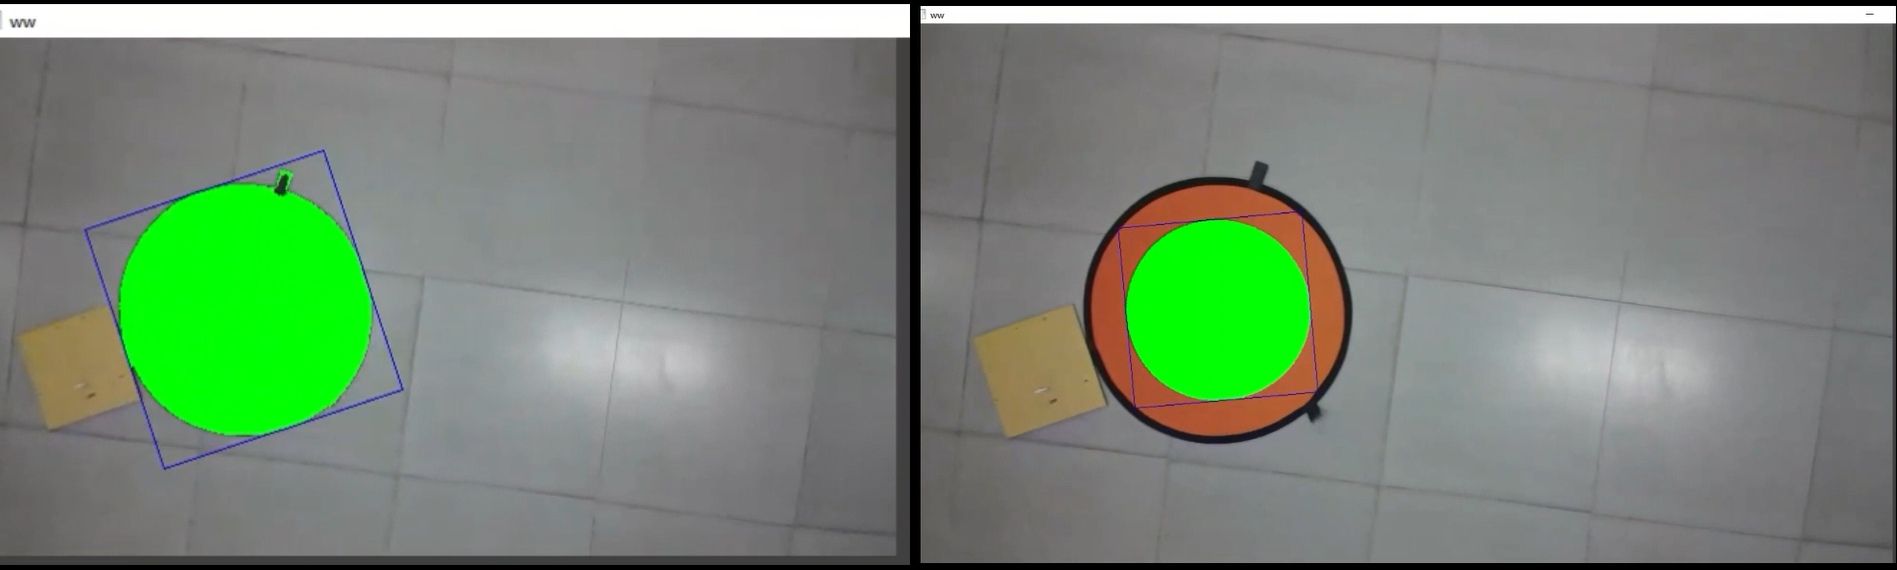
\includegraphics[width=0.8\linewidth]{./Figure/Kalman_Prediction.png}
  \caption{卡尔曼滤波器最优估计}\label{Fig:img19}
\end{figure}

将落点坐标以xy坐标系形式绘制如下,其中红色的点表示检测到的数据,预测的点是将检测到的数据进行卡尔曼滤波最优估计后的数据:

\begin{figure}[ht]
  \centering
  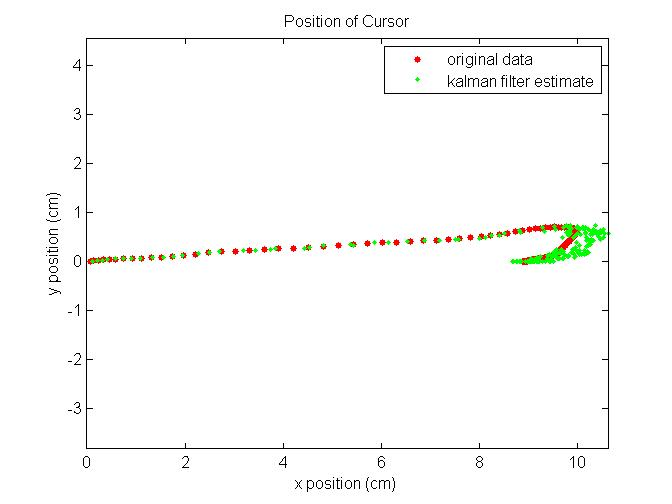
\includegraphics[width=0.8\linewidth]{./Figure/Landingpad_Kalman_Prediction.jpg}
  \caption{落点坐标对比}\label{Fig:img20}
\end{figure}


% 致谢
%!TEX root = ../Demo.tex
\begin{thanksfor}
大学本科的四年学习即将结束,感谢李隐峰副教授对于项目的指导,感谢实验室的成员的共同参与加快项目的发展。

感谢DJI大疆创新对于开发者提供的相关技术支持与帮助,我也是通过RoboMaster机甲大师赛和RoboMaster ICRA人工智能挑战赛等竞赛进一步了解到DJI大疆创新的相关产品以及其企业的创新的精神,并将它们应用于我自己的一些竞赛和项目中。感谢开源界两大教科书式项目Ardupilot和PX4,感谢世界上对于开源飞控维护的社区与团队,使得我们能从中学到很多相关的知识,了解飞控参数调试和算法优化的一些经验。同时,作为Ardupilot官方论坛的成员,我也积极参与论坛内的相关技术讨论,进一步了解当前开源飞控系统的发展趋势、硬件性能、以及相关新功能适配等。

\end{thanksfor}

%参考文献
\phantomsection                         % 生成该页的链接
\addcontentsline{toc}{chapter}{\bibname}
\bibliographystyle{gbt7714-unsrt}       % 不对参考文献排序% gbt7714-plain%对参考文献排序 
\bibliography{ThesisFiles/RefFile}      % 在正文中必须引用,才能显示对应的参考文献

% 附录部分
\appendix
%!TEX root = ../Demo.tex
\chapter{数据}

\section{代码}
\lstinputlisting[language=Java,caption={OpenCV目标检测核心代码},label=cpp]{./Code/TargetDetect.java}
%标题不编号
\lstinputlisting[language=Java,title={原版PID控制核心代码},label=java]{./Code/VisualLandingFlightControl.java}
%无行号
\lstinputlisting[language=Matlab,title={MPC控制MATLAB仿真代码},label=matlab]{./Code/MPC_Control.m}


\begin{thebibliography}{A1}
\bibitem[A1]{shanshui}
许嵩. 惊鸿一面[A]. 海蝶音乐. 不如吃茶去[C]. 北京: 北京海蝶音乐有限公司, 2014, 8.

\end{thebibliography}

\end{document}

